\documentclass[]{article}
\usepackage[UTF8]{ctex}
\usepackage[a4paper,left=10mm,right=10mm,bottom=10mm,top=10mm]{geometry}
\usepackage{graphicx}
\usepackage{float}
\usepackage{amsmath,amsfonts,amssymb,amsthm}
\usepackage{array,color}
%opening
\title{计算机科学中的数学基础--Exercise13}
\author{陈昱衡 521021910939}
\date{\today}

\begin{document}

\maketitle


\section*{Warmup5}
\begin{figure}[H]
    
    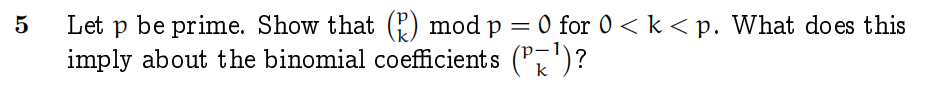
\includegraphics[scale = 0.6]{2023-03-27-17-10-45.png}
\end{figure}
将$\left( \binom{p}{k}\right)$展开,有:
\begin{align}
    \binom{p}{k}&=\frac{p \times (p-1) \times \cdots \times (p-k+1)}{1 \times 2 \times \cdots \times  (k-1) \times k}  
\end{align}
以为p为素数,所以 $p$ 无法与分母中的任何一项消去公因式,所以,最后相当于$mp$,故$\left( \binom{p}{k}\right) \bmod p = 0$.
而由式5.8,$\left( \binom{p}{k}\right)$可以拆开为:$\left( \binom{p - 1}{k}\right)$ + $\left( \binom{p - 1}{k - 1}\right)$。
由$\binom{p}{k}$ $\bmod$ $p$ = 0,故有

$\binom{p - 1}{k}$ + $ \binom{p - 1}{k - 1}$ $\bmod p $= 0;
% 故有,$\left( \binom{p - 1}{k}\right)$ $\bmod$ $p$ = $(-1)^k$
\par 
对于$k=0$,有$\binom{p-1}{k} \bmod p = 1$,因此,由于相邻两个二项式$(\binom{p-1}{k-1} + \binom{p-1}{k}) \bmod p = 0$,因此根据 $k=0$的情况,可以推出$k=1$的情况,因此,可以依次推导。最终由结论$\binom{p-1}{k} \bmod p = (-1)^k$.
\par 



\section*{Warmup6}

\begin{figure}[H]
    
    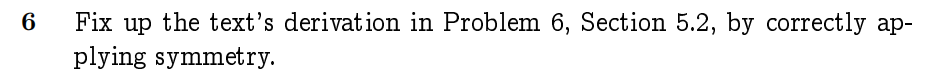
\includegraphics[scale = 0.6]{2023-03-27-17-12-02.png}
\end{figure}
观察题目,我们发现,求和式的求和范围由$k \ge 0$ 变为了$k$,因此,我们需要额外考虑这两个范围的差异.\par 
因为二项式系数$\binom{n}{k}$中,$n$无范围限制,$k$必须为非负数,因此,可以得到,我们还需考虑$k=-1$时产生的影响.\par 
$k=-1$时的项为
\begin{align}
    &\frac{1}{n+1}\binom{n-1}{n}\binom{n+1}{0}(-1)^{-1}\\
    &=\frac{(-1)^{-1}}{n+1}\binom{n-1}{n}\\
    &=\frac{(-1)^{-1}}{n+1}\frac{(n-1) \times (n-1) \times \cdots \times (n-1 - n + 1)}{n \times (n-1) \times \cdots \times 1}\\
\end{align}
故,当$n=0$时,为1,其余情况,为0.

\section*{Basics13}
\begin{figure}[H]
    
    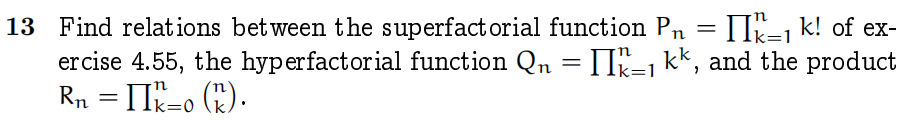
\includegraphics[scale = 0.6]{2023-03-27-17-12-20.png}
\end{figure}

写开上面三个式子,有
\begin{align}
    P_n &= \prod_{k=1}^{n}k! \\
    &=1! \times  1 \times 2 \times \cdots \times n!\\
    &= 1^{n} \times 2^{n-1} \times 3^{n-2} \times \cdots \times (n-1)^2 \times n\\
    Q_n &= \prod_{k=1}^{n}k^k\\
    &= 1^1 \times 2^2 \times \cdots \times (n-1)^{n-1} \times n^n\\
    R_n &= \prod_{k=1}^{n}\binom{n}{k}\\
    &=\frac{n}{1} \times \frac{n \times (n-1)}{1 \times 2} \times \frac{n \times (n-1) \times (n-2)}{1 \times 2 \times 3} \times \cdots \times \frac{n \times (n-1) \times \cdots \times (n-k+1)}{1 \times 2\times \cdots \times k}\\
    &=\frac{n^n \times (n-1)^{n-1} \times \cdots \times 1}{1^{n} \times 2^{n-1} \times \cdots \times n}\\
    &=\frac{Q_n}{P_n}
\end{align}

故,有$R_n = \frac{Q_n}{P_n}$.

\end{document}